\documentclass[a4paper,11pt]{article}
\usepackage[utf8]{inputenc}
\usepackage{algorithmic}
\usepackage{algorithm}
\usepackage{pst-plot}
\usepackage{graphicx}
\usepackage{endnotes}
\usepackage{graphics}
\usepackage{floatflt}
\usepackage{wrapfig}
\usepackage{amsfonts}
\usepackage{amsmath}
\usepackage{verbatim}
\usepackage{hyperref}
\usepackage{multirow}
\usepackage{pdflscape}
 \usepackage{enumitem}

\usepackage{hyperref}
\hypersetup{pdfborder={0 0 0 0}}

\pdfpagewidth 210mm
\pdfpageheight 297mm 
\setlength\topmargin{0mm}
\setlength\headheight{0mm}
\setlength\headsep{0mm}
\setlength\textheight{250mm}	
\setlength\textwidth{159.2mm}
\setlength\oddsidemargin{0mm}
\setlength\evensidemargin{0mm}
\setlength\parindent{7mm}
\setlength\parskip{0mm}

\newenvironment{exercise}[3]{\paragraph{Exercise #1: #2 (#3pt)}\ \\}{
\medskip}
\newcommand{\question}[2]{\setlength\parindent{0mm}\ \\$\mathbf{Q_#1:}$ #2\ \\}

\author{\large{Aqeel Labash, Daniel Majoral, Raul Vicente}}
\title{\huge{Introduction to Computational Neuroscience}\\\LARGE{Practice on Single Neuron Models}}

\begin{document}
\maketitle

\textbf{A request:} Please track how long it will take to complete this set of exercises. Add this time to your final report.
\ \\
\textbf{NOTE:} In this homework you are required to also submit your code.\\
\textbf{NOTE:} If you are not using Matlab/Octave, you will unfortunately need to rewrite the code in your preferred language. In the beginning of the course we warned this will happen eventually. But consider also doing this session in Matlab/Octave, as not much knowledge of the language is required for these tasks - just replace some values here and there.\\
\ \\
\ \\
%
% Intro
%
In this session we will have a brief look on three different computational models of a neuron: McCulloch-Pitts, Intergrate-and-Fire and Hodgkin-Huxley.\

\ \\

%
% Logic gates
%
\begin{exercise}{1}{Logic gates}{1}
On the lecture we have seen how to construct \texttt{AND}, \texttt{OR} and \texttt{NOT} logic gates using the the McCulloch-Pitts model of a neuron. Remember that:\\
 \texttt{if sum(w.*x)<0, output is 0}\\
 \texttt{if sum(w.*x)>=0, output is 1} (notice that 0 is included)\\
 Your task is to construct more logical operations using MP neurons. Please construct the following two gates:
\begin{enumerate}
\itemsep 0em
	\item \texttt{NAND}
	\item \texttt{XOR}
\end{enumerate}
\textbf{HINT 1} For the \texttt{XOR} gate you will need more than one neuron.\\
\textbf{HINT 2} Same input can go simultaneously to several neurons (and with different weights).
\textbf{HINT 3} You can see how \texttt{XOR,NAND} behave in  \href{https://en.wikipedia.org/wiki/Logic\_gate}{https://en.wikipedia.org/wiki/Logic\_gate}.
\end{exercise}

%
% Integrate and Fire
%
\begin{exercise}{2}{Integrate and Fire neuron model}{2.5}

Integrate-and-Fire neuron (IAF neuron) accumulates voltage until it reaches the \emph{threshold}. After that it outputs/emits a spike and resets the voltage back to the reset value. In this exercise we will model the behaviour of IAF neurons and study their properties. We will add features and behaviours to our model step by step. \\ 

The file \texttt{code/integratefire.m} contains first of all some theoretical explanation of how we are going to simulate a neuron's behaviour (read it!) by numerically solving the differential equation governing integrate-and-fire neuron.\\ \textbf{Your task is} to complete the series of \texttt{TODO}-s in the \texttt{integratefire.m}. You need to complete these TODO-s one by one in the given order and report \textbf{ALL} figures, answers, interpretations and conclusions you will make during the work.\\

\textbf{You will need to:}\\
\begin{enumerate}
\item \texttt{TODO 1}: write how to calculate V(2), given V(1), I and C
\item \texttt{TODO 2}: write how to calculate V(3), given V(2), I and C
\item \texttt{TODO 3}: write how to calculate V(t+1), given V(t), I and C. Plot what happens and describe (describe in comparison with TODO 4)
\item \texttt{TODO 4}: replace the 0 with the conditional sentence to check if V(t) is above the threshold level Vth. Plot what happens. Describe, compare.
\item \texttt{TODO 5}: replace the 0 with an expression that would add 1 to $number\_of\_spikes$. Run the for loop again, report the count with default values.
\item \texttt{TODO 6}: increase the current to 10.0. Plot the behaviour and report the count.
\item \texttt{TODO 7}: Try also other currents, observe the spike count (no need to plot Vm(t) for each current). Plot it in your head and/or on a graph. What is the relationship - exponential? logarithmic? linear? less than linear?
\item \texttt{TODO 8}: add the term $noise*sqrt(dt)*randn $ to the V(t+1) equation. This input reflects he fact that neurons always receive random inputs from their neighbours. Observe the noise on Vm plot.
\item \texttt{TODO 9}: This \texttt{TODO} has its separate part of code below the for loop used so far. Your task is to change the noise level and plot 3 different raster plots (10 trials on each) with different noise levels. Instructions are at the end of the file.
\end{enumerate}

\ \\
One of the outputs should look something like this
\begin{figure}[H]
   \centering
   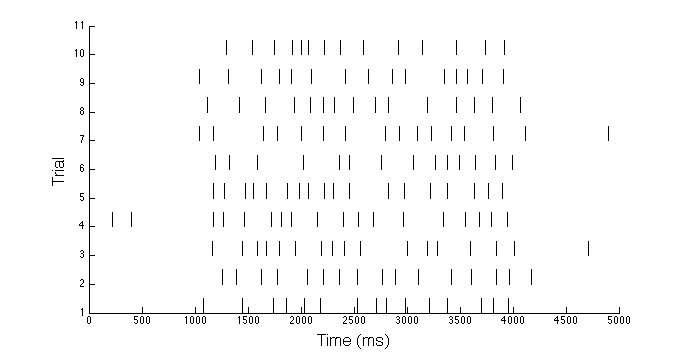
\includegraphics[width=0.8\textwidth]{raster_plot.png} 
   \caption{10 trials of data generated using Integrate-and-Fire neuron model.}
   \label{fig:rasterplot}
\end{figure}
\end{exercise}



% Integrate and Fire with synapses
%
\begin{exercise}{3}{Integrate and fire advanced}{1.5}

In this exercise we will play with somewhat more realistic versions of integrate-and-fire model.\\

In first stage we add a leak current to the neuron. This current is caused by the ion pumps and it drives the membrane potential slowly towards its resting state. In the previous exercise there was no such current - when the input current stops, the potential remains fixed at the current value. With leak current added, the Vm now slowly returns to its resting state at -70 mV.\\
Another difference is that beforehand any current, no matter how small, would eventually drive the neuron to spike. In the current exercise however, weak inputs are balanced out by the leak current.\\

The code you have to read, understand and modify is in \texttt{leakyintegratefire.m}\\

Your task is to:
\begin{itemize}
\item find the lowest $I_{injected}$ (with 0.1 precision) that leads to a spike. Plot the behaviour at this \textbf{I} value and at the value 0.1 below (last one with no spike). Describe what happens. Describe also what happens after the stimulus is turned off.
\item How does firing rate (spikes per second) differ at I = 5.0, 10.0, 25.0, 50.0 with and without (results in TODO 7 in previous exercise) leak current? 
\end{itemize}

In the second stage we explore the neuron's behaviour if it receives input from incoming (\emph{presynaptic}) spikes rather than constant injected current. Even though one incoming signal is not enough to activate our neuron, \emph{temporal summation} of inputs happening in a short period of time can lead to the voltage reaching the threshold. The code you need to understand and modify is provided in \texttt{integratefiresynapses.m}.\\

For this task you have to remember that if a neuron gets enough excitatory input in a short period of time, it will activate. The same amount of inputs dispersed over a longer period will not lead to firing. Your task is again to modify code near the \texttt{TODO} signs and to answer some questions:
\begin{enumerate}
	\item \texttt{TODO 1} The neuron only receives one incoming spike at t=300ms. Plot the membrane potential and the strength of the synaptic current in time. i) Describe how membrane potential and strength of current change over time (peak values, shape). ii) How long does it take for the current to decrease by half (half-life)? How is that related to the "taus" parameter? iii) Modify the strength of the synaptic current up to a point where one presynaptic spike is enough to produce a postsynaptic spike.
	\item \texttt{TODO 2} Uncomment the line and the neuron will receive a spike every 50ms. Nevertheless it never fires. Why?
	\item \texttt{TODO 3} Uncomment the line and replace t3 (time of third spike) with a number bigger than 101. What is the lowest value for t3 so that the receiving neuron does not emit a spike?
\end{enumerate}
\end{exercise}


%
% Hodgkin-Huxley
%
\begin{exercise}{4}{Hodgkin-Huxley neuron model}{1.5}

Hodgkin-Huxley model is considered to be the most important computational neuronal model in the neuroscience today. We have the model already implemented in the file \texttt{HH0.m}, study it. Follow the instructions in the \texttt{hodgkinhuxley.m} file and report all figures, thoughts, interpretations and conclusions you will have during the work.\\

The \texttt{TODO} marker will indicate places where you have to do something: complete the code, plot and report a figure, give an interpretation, etc.
\begin{enumerate}
\item Explain the nature of m, h and n in terms of Na+ and K+ ion channels being open or closed (discussed in lecture).
\item Add the figure at I0=5.0 to the report. Modify I0 and report the lowest I0 that still causes a spike in the beginning of simulation. And the lowest I0 that causes continuous spiking till the end of simulation. (Precision of your answer should be at least 0.1)
\item Count the number of spikes at different I0 values (code provided). \textbf{Note that} this series of simulations can take up to 5-10 min, do not panic if it takes time. Describe what you see. Why this \textit{input-output curve} is more biologically realistic than the input-output relation of IAF? How is the non-linearity of the relationship related to modelling the ion channels and not simply resetting the membrane potential instantaneously as soon as threshold is reached? 
\end{enumerate}
\end{exercise}


\begin{exercise}{5*}{Bonus}{0.5}
We take the freedom to award bonus points for the appearance of the report. Some reports are really badly formatted and hard to read. So we want to reward people who make their reports more readable and our life more pleasant.
\end{exercise}


\ \\
\ \\
\ \\
\ \\

Please submit a \texttt{pdf} report with answers to the questions and comments about your solutions. Include figures, explanations. \textbf{Include the completed code files and zip the files together.} The code files are not the place to answer questions, answers must also be contained in the pdf. Upload it on the practice session page on the course website.

\end{document}










